\chapter{Logic internal representation}
\label{chap:LogicInternalRepresentation}

In this chapter every element of \gls{FOL} will be described in context of implementation along with some computational complexity adnotations.

\section{First Order Logic elements}

\begin{figure}[H]
\begin{centering}
  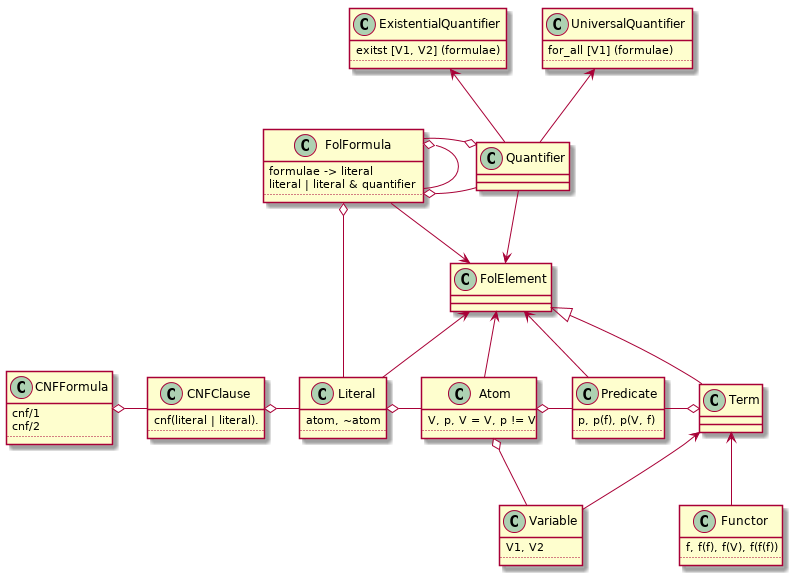
\includegraphics[width=\textwidth]{logic-formula-generator/fol/fol_elements.png}
  \caption{Class diagram for FOL}
\end{centering}
\end{figure}

\subsection{Functor}

Functor can contain variable or another functor.
Given that
$n$ is functor recursion depth,
$a$ is functor arity,
$f(n, a)$ number of functor signatures can be produced.

\begin{align}
	&f(n, a) =
	\begin{cases}
		a, \text{for } n = 0, \\
		a \sum_{i=n}^{i=1} \sum_{j=a}^{j=0} f(n-i,a-j) \\
	\end{cases}
\end{align}

Given that functor arity $a_f$ is in range $[a_{fmin}, a_{fmax}]$  and maximal recursion depth is $n_{max}$, $f(n_{max}, a_{fmin}, a_{fmax})$ number of functor signatures can be produced.

\begin{align}
	f(n_{max}, a_{fmin}, a_{fmax}) = \sum_{i=0}^{n_{max}} \sum_{j=a_{fmin}}^{a_{fmax}} f(i, j),
\end{align}

\subsection{Predicates}

Predicates can contain functors or variables.
Given that $a_p$ is predicate arity, $P(a_p)$ number of predicate signatures can be produced.

\begin{align}
	P(a_p) &=
	\begin{cases}
		1, \text{for } a_p = 0 \\
		(f(n_{max}, a_{fmin}, a_{fmax}) + 1)^{a_p}, \\
	\end{cases}
\end{align}

Given that predicate arity $a_p$ is in range $[a_{pmin}, a_{pmax}]$, $p(a_{fmin}, a_{fmax})$ number of functor signatures can be produced.

\begin{align}
	p(a_{pmin}, a_{pmax}) = \sum_{i=a_{pmin}}^{a_{pmax}} p(i),
\end{align}

\subsection{Atoms}

Atom can contain variabe or predicate. Atom connects items with binary mathematical connective: $=$ or $!=$ or $\emptyset$ (no connective).
Given that atom $connective$, $A(connective)$ atom signatures can be produced.

\begin{align}
	A(connective) &= 
  \begin{cases}
    (p(a_{pmin}, a_{pmax}) + 1)^{2}, \text{for } connective \in \{'=', '!='\} \\
    p(a_{pmin}, a_{pmax}) + 1, \text{for } connective \in \{\emptyset\}
  \end{cases}
\end{align}

\subsection{Literals}

Literal is atom or its negation.

\begin{align}
  L = A(AllowedConnectives) * 2
\end{align}

\subsection{CNF Clause}

Clause $C$ can contain only literals $L$. The order of literals is irrelevant $C = \{l1, 12, \dots\}$

Given that 
clause length $l$ and 
set of unique literals $L = \{l1, l2, \dots\}$, $\forall_{i,j \in L} i \neq j$
$C(l)$ clauses can be produced.

\begin{align}
  C(l) = \binom{L}{l},
\end{align}

Given that clause length $l$ is in range $[l_{min}, l_{max}]$

\begin{align}
  C(l) = \sum_{i=l_{min}}^{i=l_{max}} C(i)
\end{align}

\subsection{CNF formulas}

Given that
formula contains $c$ clauses and
set of unique clauses $C = \{c1,c2, \dots\}$
$F$ formulas can be produced.

\begin{align}
	&F_{cnf}(x) = \binom{|C|}{x}
\end{align}
